\documentclass{article}

\usepackage[main=english,vietnamese]{babel}
\usepackage[T1]{fontenc}
\usepackage[utf8]{inputenc}
\usepackage[sexy]{evan}
\usepackage{matchsticks}
\usepackage{wrapfig}
\usepackage{listings}

\newtheorem{hint}{Hint}

\title{A picture is worth a thousand words - Part 3}
\author{Nghia Doan}
\date{\today}

\begin{document}

\maketitle

This article is the third part of the series on investigating a number of ways to \textit{prove area equality without writing lengthy proof.}

\begin{example*}[Example 11]
    In the convex quadrilateral $ABCD,$ $E, F, G,$ and $H$ are midpoints of $AB,$ $BC,$ $CD,$ and $DA,$ respectively.
    $EG$ and $FH$ intersect at $I$.
    Prove that
    \[
        [EBFI] + [GDHI] = \half [ABCD].
    \]
\end{example*}

\begin{figure}[h]
    \centering
    \begin{minipage}[t]{6.5cm}
        \begin{center}
            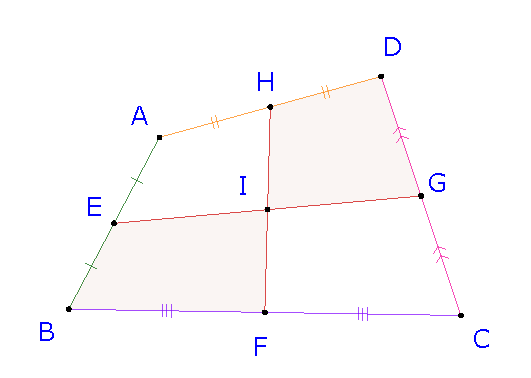
\includegraphics[width=6.5cm]{./svg/pdf/23-24-s3-i-p12.pdf}
        \end{center}
    \end{minipage}
    \qquad
    \begin{minipage}[t]{6.5cm}
        \centering
        \begin{center}
            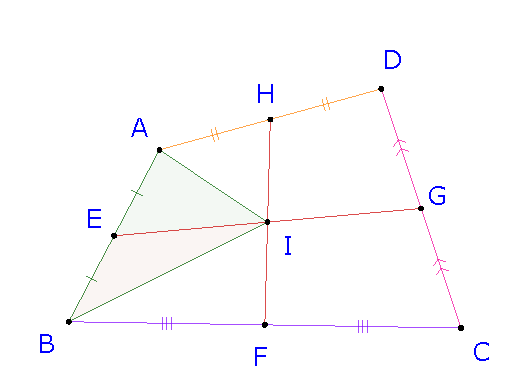
\includegraphics[width=6.5cm]{./svg/pdf/23-24-s3-i-p12-s.pdf}
        \end{center}
    \end{minipage}
\end{figure}

\begin{proof}
    Connect $AI.$ Since $E$ is midpoint of $AB,$ thus the triangles $AEI$ and $EIB$ have the same area.
    Similarly the area of $BIF$ and $CFI$ are the same. Thus $[EBIF] = \half [ABCI].$
    Similarly $[GDHI] = \half [CDAI].$
    Summing up, we have $[EBFI] + [GDHI] = \half [ABCD].$
\end{proof}

\newpage

\begin{example*}[Example 12]
    $ABCD$ is a trapezoid. $E, F$ are arbitrary points on $BC$ and $AD,$ respectively.
    $AE, BF$ intersect at $G$ and $CF, DE$ intersect at $H.$ Prove that:
    \[
        [ABG] + [CDH] = [EFGH].
    \]
\end{example*}

\begin{figure}[h]
    \centering
    \begin{minipage}[t]{6.5cm}
        \begin{center}
            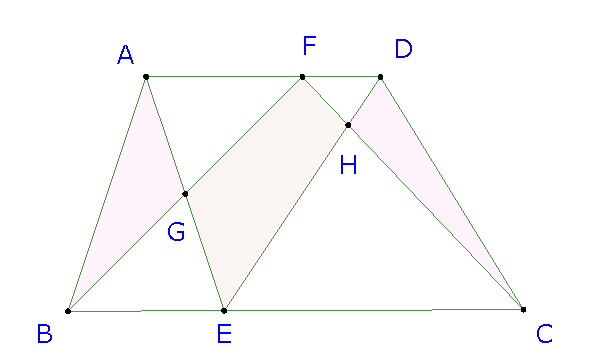
\includegraphics[width=6.5cm]{./svg/pdf/23-24-s3-i-p13.pdf}
        \end{center}
    \end{minipage}
    \qquad
    \begin{minipage}[t]{6.5cm}
        \centering
        \begin{center}
            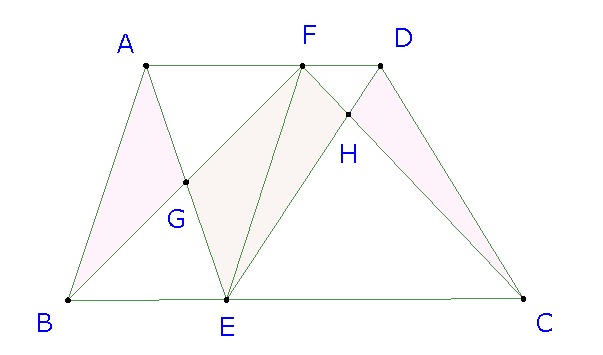
\includegraphics[width=6.5cm]{./svg/pdf/23-24-s3-i-p13-s.pdf}
        \end{center}
    \end{minipage}
\end{figure}

\begin{proof}
    Connect $EF.$ Since $BE$ parallel with $AF$ so $[ABF] = [AEF],$ thus $[ABG] = [FEG].$
    Similarly $[CDH]=[FEH].$
    Summing up, we have $[ABG] + [CDH] = [EFGH].$
\end{proof}

\begin{example*}[Example 13]
    $ABCD$ is a rectangle. $E, F$ are midpoints of $AB, AD,$ respectively.
    $CE, BF$ intersect at $G.$ Prove that:
    \[
        [AEGF] = [BGC].
    \]
\end{example*}

\begin{center}
    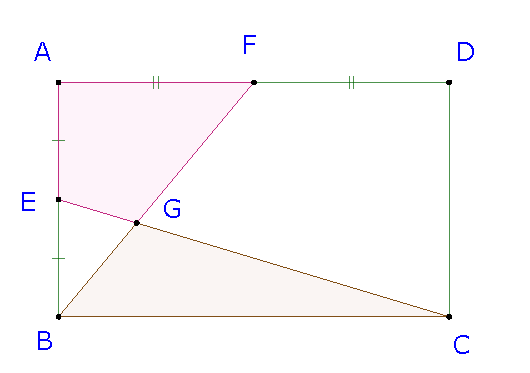
\includegraphics[width=6.5cm]{./svg/pdf/23-24-s3-i-p14.pdf}
\end{center}

\begin{proof}
    It is easy to see that the triangles $ABF$ and $EBC$ have the same area 
    \[
        \begin{aligned}
            &[ABF] = \frac{AB \cdot AF}{2} = \frac{AB \cdot AD}{4},\ [EBC] = \frac{EB \cdot BC}{2} = \frac{AB \cdot AD}{4}\\
            &\Rightarrow [AEGF] = [ABF] - [EBG] = [EBC] - [EBG] = [BGC].
        \end{aligned}
    \]
\end{proof}

\newpage

\begin{example*}[Example 14]
    $ABCD$ is a rectangle. $E, F$ are arbitrary points on of $CD, DA,$ respectively.
    $AE$ intersects $BF,$ $BE$ at $G, H,$ respectively. $CF$ intersects $BE$ at $I.$ Prove that:
    \[
        [AGF] + [FHED] + [CEI] = [BGHI].
    \]
\end{example*}

\begin{center}
    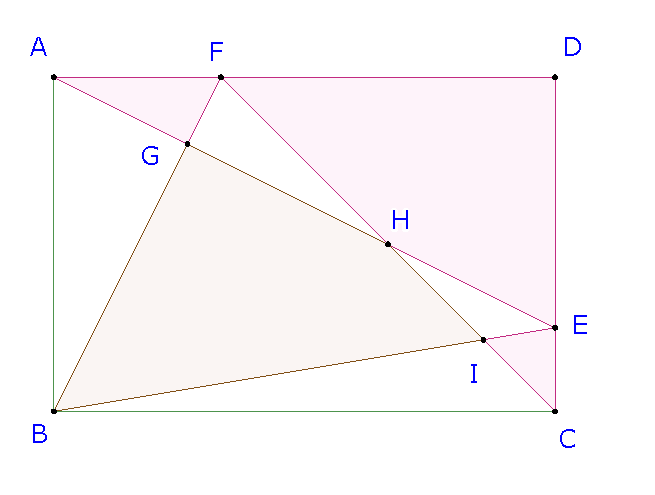
\includegraphics[width=6.5cm]{./svg/pdf/23-24-s3-i-p15.pdf}
\end{center}

\begin{proof}
    It is easy to see that the triangles $BDF$ and $CDF$ have the same area, similarly the triangles $BDE$ and $ADE$ have the same area, therefore:
    $[BFDE] = [CDF] + [ADE].$ But
    \[
        \begin{aligned}
            [BFDE] &= [BGHI] + [GFH] + [FHED] + [HIE],\\
            [CDF] + [ADE] &= [AGF] + [GFH] + 2 [FHED] + [HIE] + [CEI]\\
        \end{aligned}
    \]
    Hence, $[BGHI] = [AGF] + [FHED] + [CEI].$
\end{proof}

\begin{example*}[Example 15]
    $ABC$ is a quarter of circle. $D, E$ trisect arc $\arc BC$: $\arc CD = \arc {DE} = \arc {EB}.$
    Prove that the blue circular sector $ACD$ and the red region $DEGF$ have the same area.
\end{example*}

\begin{figure}[h]
    \centering
    \begin{minipage}[t]{6.5cm}
        \begin{center}
            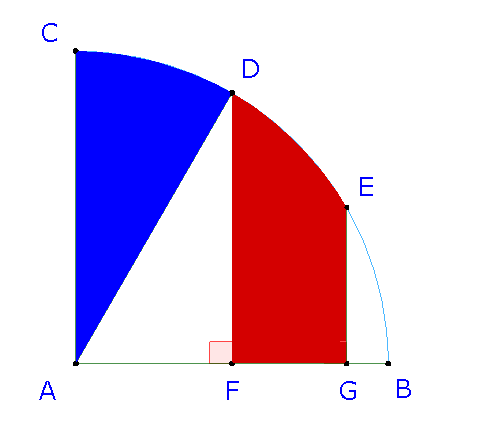
\includegraphics[width=5.5cm]{./svg/pdf/23-24-s3-i-p16.pdf}
        \end{center}
    \end{minipage}
    \qquad
    \begin{minipage}[t]{6.5cm}
        \centering
        \begin{center}
            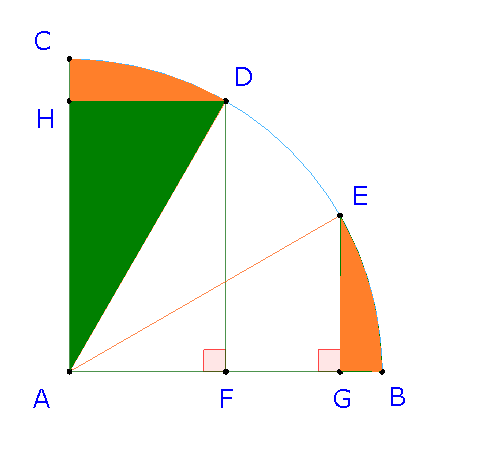
\includegraphics[width=5.5cm]{./svg/pdf/23-24-s3-i-p16-s.pdf}
        \end{center}
    \end{minipage}
\end{figure}

\begin{proof}
    Since $D, E$ trisect arc $\arc BC,$ the circula sector $ACD$ and $AEB$ are congruent.
    Thus, if $DH \perp AC,$ then the orange regions $CDH$ and $EGB$ are the same.
    It is easy to see that $\triangle AHD \cong \triangle ADF,$
    thus the sum of the area of $\triangle ADF$ and the region $EGB$ is the same as the blue circular sector $ACD$.
    This means that the area $DEGF$ is one-third of the quarter circle $ABC,$ thus it is the same as the area of the blue circular sector $ACD$
\end{proof}

\end{document}